\subsection{GraphDrawer}
To solve the problem of letting students visually answer questions, the GraphDrawer Vue component was created. GraphDrawer can be included on any page where data structures should be displayed. It is built as a layer on top of the HTML5 Canvas element.
\\[11pt]
The GraphDrawer includes a rendering engine which is responsible for converting a part of the world to an image displayed to the user. The world is where every node and edge is placed before they can be rendered. A rendering engine is software which generates graphics from data. The world contains everything the user can interact with. The interaction is done through the HTML5 Canvas element. User interaction events are received from the canvas element in the form of "The user clicked at this (x, y) position," or "The user currently has two fingers on the screen at (x1, y1) and (x2, y2)". The GraphDrawer needs to convert the screen coordinates to world coordinates, and then decide if the given event at the given world position has any meaning for the state of the world. The coordinate conversion is done by the camera.
\\[11pt]
The world consists of two types of entities, nodes (vertices) and edges. Entities are stored in arrays on the GraphDrawer object. Nodes are drawn as either a circle or a square. A node needs to specify its position in the world, which is stored on the node object as the properties \code{x} and \code{y}. It also needs to store information about how large it is, which is stored in the \code{w} and \code{h} properties. If the node is a circle, then \code{w} and \code{h} should have the same value, and the value should be the circle radius. If it is an ellipse, then the \code{w} is the radius along the x-axis, and the \code{h} is the radius along the y-axis. A node needs a value, stored in the \code{v} property. This can be text, a number, or a combination of text and numbers. GraphDrawer will only render nodes if they have the \code{x}, \code{y}, \code{w}, \code{h} and \code{v} properties. There are also several optional properties a node can have. \code{selected} is a boolean used by a controller to indicate whether a node has been selected (\code{true}) or not (\code{false}). \code{culled} is a boolean used by the camera to indicate whether a node should be drawn (\code{false}) or not (\code{true}). \code{fillColor} decides what color is used to render the inner part of the node. If it is undefined, white is used. \code{strokeColor} decides what color will be used to render the outline of a node. If it is undefined, black is used.
\\[11pt]
Edges are used to link nodes together. An edge needs to have two properties, \code{n1} and \code{n2}, which are references to the nodes being linked by the edge. Edges are drawn as either a line or an arrow, between the two nodes. If the edge has the property \code{directed} with the value \code{true}, an arrow is drawn pointing from \code{n1} at \code{n2}. If \code{directed} is \code{false} or \code{undefined}, a line is drawn. The \code{strokeColor} property decides which color will be used to draw the line/arrow. If it is undefined, black is used. An edge can also have the \code{v} property. \code{v} represents the cost of going from \code{n1} to \code{n2} (and from \code{n2} to \code{n1} if \code{directed} is \code{undefined} or \code{false}). \code{v} should be a number, and its value is drawn next to the line/arrow.
\\[11pt]
To render the world, three objects are needed, the world, a camera, and a HTML5 canvas. The world has information about the entities. The camera is used to decide which entities need to be drawn to the canvas. Two additional canvases are created, such that drawing the world is easier. The drawing buffer \code{drawBuffer} and the static buffer \code{staticBuffer}. The drawing buffer size is five times greater than the canvas, and the static buffer is the same size as the canvas. These objects are needed because the world might be larger than what is possible to display on a single webpage. The canvas decides how much of the webpage is used to render the world. The camera can then be moved around to display different parts of the world. When the GraphDrawer starts, an interval is started which lets the GraphDrawer update 60 times every second. Each time the GraphDrawer has the opportunity to update is called a frame. Because the application is designed to be used by both phones and computers, computationally expensive and time-consuming operations should be avoided if possible. For this reason, the GraphDrawer will often discard frames. Discarding frames means that no operation is performed, even though the opportunity to do something was there. The update function is called once per frame. If the \code{dirty} property is \code{false}, the frame is discarded. The GraphDrawer will only set the \code{dirty} property to \code{true} once, at startup, so the initial state is rendered. Afterward, a controller has to tell the GraphDrawer to not discard the next frame by setting \code{dirty} to \code{true}. The \code{dirty} property makes it possible to have a responsive user interface, and save CPU time at the same time. When a frame is not discarded, the world is redrawn. This is done in several steps:
\begin{enumerate}
    \item The canvas is cleared. This is done to prevent entities from appearing at two positions at the same time.
    \item Nodes and edges are drawn to a drawing buffer (\code{drawBuffer}). This is done by the GraphDrawer.
    \item The user interface is drawn to a separate buffer (\code{staticBuffer}). This is done by the GraphDrawer if the \code{operatingMode} is set to \code{Presentation}, or by a controller if the \code{operatingMode} is set to \code{Interactive}. \code{operatingMode} is used by the GraphDrawer and by controllers to decide what kind of user interaction is allowed.
    \item \code{drawBuffer} and \code{staticBuffer} is drawn to the canvas.
\end{enumerate}
Some users of the site could be using old hardware or somehow restrict the performance of their browser. The GraphDrawer is designed to update 60 times per second. This means that every frame is allocated: $ 1000 / 60 = 16.666... $ milliseconds to do the work. If the frame uses more than the allocated time, the user will experience this by having the program not respond for some time. If this happens, then the next frame is discarded, to give the computer time to catch up again. 60 frames per second were picked to balance how smooth the graphics move, and the program performance. If more than ten frames need more than the allocated time, the number of frames per second is lowered by 25\%. By lowering the number of frames per second, the user will still have a responsive program. The movement of the graphics looks normal unless the time per frame is increased significantly.
\\[11pt]
The drawing buffer is used to prevent screen tearing. Screen tearing happens when the world is updated in the middle of drawing the world to the canvas. The result is that some parts of the canvas show the old state of the world, while other parts show the new state. By using a separate buffer for drawing, the user will be shown a complete image of the world at every frame, instead of one which is in the process of being drawn. The user interface uses another buffer because it makes it easier to draw the interface on top of the world, by simply placing the draw statement after the world draw statement. The \code{staticBuffer} uses canvas coordinates to draw, which needs fewer operations to consistently place the interface inside the camera view.
\\[11pt]
To let the user interact with the world, two event listeners are attached to the canvas. \code{mousedown} is used to respond to mouse clicks, and \code{touchstart} is used by touch screens. These listeners use the same callback function. The callback function passes the event to the right handler, depending on handler priority. A handler is a function which takes the event as an argument and returns whether or not it consumed the event. If the event was consumed, it should not be given to any other handler. The priority of the user interface handler should generally be higher than the world handler, but the order is not forced. The GraphDrawer first checks if the user interacted with one of the buttons. If not, then a controller is given the chance to handle the event. Finally, the event is given to the gesture handlers. Gesture handlers are responsible for detecting patterns in user interaction and check if they match a given gesture. The GraphDrawer implements two gestures, pan and zoom. Pan is used to move the camera around the world. A pan gesture happens when the user clicks a mouse button and moves the pointer without releasing the button. This can also happen if the user drags their finger across the canvas. The movement must be larger than a given threshold before the camera starts moving. A zoom gesture is defined as the user dragging two fingers in opposite directions. If the fingers move towards each other, the zoom decreases. If the fingers move away from each other, the zoom increases. The average point between the fingers will remain at the same position relative to the canvas edge. The position of events is stored in different properties of the event object, depending on what type of event it is. To make it simpler to write code that works with all types of events, a helper function \code{setEventOffset} was created to convert event positions to a common format. This function should be used right after receiving an event object, to be sure the position of the event is available in the expected properties.
\\[11pt]
The GraphDrawer constructor takes four arguments, \code{canvas}, \code{locale}, \code{config} and \code{window}. \code{canvas} should be a reference to the HTML Canvas which will be used. \code{locale} should be an object containing references to all of the displayed strings in a given language. \code{config} should be an object containing configuration options. \code{window} should be a reference to the browser window object. The following is a list of all the configuration options available:
\begin{enumerate}
    \item \code{nodeShape}, determines the shape which is used to render the nodes. Possible values are \code{"Circle"} and \code{"Rectangle"}. If no value is given, \code{nodeShape} is set to \code{"Rectangle"}.
    \item \code{controlType}, determines which controller is used by the GraphDrawer. Possible values are the names of the controllers as a string. If no value is given, \code{controlType} is set to \code{"Sort"}.
    \item  \code{operatingMode}, determines if the user can manipulate the world, or view a list of states. Possible values are \code{"Interactive"} and \code{"Presentation"}. If no value is given, \code{operatingMode} is set to \code{"Interactive"}.
    \item \code{displayEdgeValues}, enables the \code{v} (value) property of edges. The value will be drawn next to the edge and can be modified if the \code{operatingMode} is set to \code{"Interactive"}. If no value is given, \code{displayEdgeValues} is set to \code{true}.
    \item \code{directedEdges}, enables drawing of edges as arrows instead of lines. If it is set to \code{true} then all edges which does not have the \code{directed} property set to \code{false} are drawn as an arrow instead. If no value is given, \code{directedEdges} is set to \code{false}.
\end{enumerate}
To determine the position and size of a canvas, it is not enough to define the size in the CSS. If the size defined by the CSS is different from the width and height properties of the canvas, the image will be stretched to fit the size defined by the CSS. Because the application is going to be used by screens of any size, the canvas size needs to scale with the screen size. To achieve this, the update function will check if the width of the canvas matches the \code{clientWidth} property. The \code{clientWidth} property is how much space the canvas has been given on the screen. If they do not match, then the size properties of the canvas need to be changed. The width is set to the same value as \code{clientWidth}. The height is determined by the screen aspect ratio and the canvas width. By using the aspect ratio, the canvas has a greater height than width on mobile devices, and a smaller height on computers.
\\[11pt]
When the size of the canvas is changed, the size of the \code{drawBuffer} and \code{staticBuffer} also need to change. Because they are also canvases, this is simply done by updating the width and height properties. After the width or height property of a canvas is changed, any data drawn to it is cleared. The \code{drawBuffer} can be fixed by setting the \code{dirty} value to \code{true}, because this will make the GraphDrawer redraw the world. The \code{staticBuffer} is usually not redrawn every frame, e.g., the buttons to navigate between algorithm steps, and is not part of the draw function. To redraw the \code{staticBuffer}, every object on it needs to get a new position and be redrawn right after changing the canvas size. The camera keeps a reference to the size of the canvas in its \code{viewportHeight} and \code{viewportWidth} properties. If these are not changed, the resulting image is stretched. 
\\[11pt]
After resizing the canvas, the \code{drawBuffer} can be too large, if the user has a screen with a very large resolution, e.g., above 4K. Browsers have different limits, but based on numbers from Mozilla \cite{CanvasMaxSize} and Chromium \cite{CanvasMaxSizeChromeium}, modern browsers have a width and height limit of 32767 pixels for the canvas element. If this limit is exceeded then depending on the browser, the canvas can stop working, the site can stop working, or the browser can crash. The actual limit seems to be much lower than 32767 pixels. The canvas slowed down significantly when the width was larger than 7000 pixels, and completely stopped working when the width was larger than 8500 pixels. The website was viewed on a modern version (v73.0.3683.103) of the Chrome browser. To be sure that the size of the canvas won't prevent the GraphDrawer from working, a limit of 7000 pixels has been implemented.
\\[11pt]
The position of an arrow from one node to another node depends on the shape of the node it is pointing at. If the node is a circle, then the arrow is drawn at the circumference. This is done by creating a line between the two nodes and checking where it intersects the circle. Rectangle nodes have four defined positions for the arrow, one at the center of every edge. To figure out which point to use, the angle (in degrees) between the nodes is used. The angle is calculated from the x-axis and increases counterclockwise. The edge is picked based on the following criteria:
\begin{enumerate}
    \item If the angle is between 45 and 135 degrees, the point at the top edge is picked.
    \item If the angle is between 135 and 225 degrees, the point at the left edge is picked.
    \item If the angle is between 225 and 315 degrees, the point at the bottom edge is picked.
    \item If no edge has been picked, the point at the right edge is picked.
\end{enumerate}
Developers can add or remove features from the GraphDrawer by creating controller objects. Controller objects are used to modify the user interaction and the world presentation. They can interrupt the GraphDrawer at pre-determined states. It is also possible to create custom interrupts by creating timers (\code{setTimeout}, \code{setInterval}) or by adding event handlers to the canvas object. The controller interface is simple by design and only requires two methods. There are also some optional methods which can be implemented to add more functionality.
\begin{figure}[H]
    \centering
    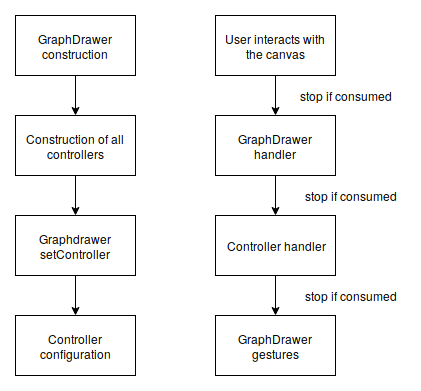
\includegraphics[width=0.5\linewidth]{/graphdrawer/controllerlifecycle}
    \caption{Graphdrawer - controller interaction}
    \label{fig:graphdrawerControllerLifeCycle}
\end{figure}
\begin{enumerate}
    \item Required: The controller constructor. The constructor should take two arguments. The first being a reference to the GraphDrawer, and the second being an optional configuration object.
    \item Required: \code{export()}, should return an object. The \code{export} method is called when the system wants to retrieve an answer or solution from the GraphDrawer. The returned object should be a representation of the world, which can be understood by one of the algorithm implementations, or by a solution checker function.
    \item Required: \code{mouseDownHandler(e)}, should return \code{true} or \code{false}. The \code{mouseDownHandler()} is called when the user clicks or touches the canvas. It is called with the event as the first and only argument. \code{mouseDownHandler()} should return \code{true} if the event was handled and should be consumed, or \code{false} if it was ignored.
    \item Optional: \code{configure()}. If the controller was given a configuration object at instantiation, then the \code{configure()} method should be implemented. It is called when the GraphDrawer changes controller.
    \item Optional: \code{dirtyUpdate()}. \code{dirtyUpdate()} is called right before the world is rendered and drawn to the screen.
    \item Optional: \code{parseSteps()} and the \code{steps} property. If the \code{operationMode} of the GraphDrawer is set to \code{"Presentation"}, then the controller is expected to have a list of steps in the \code{steps} property of the controller. The user can navigate through the list. \code{parseSteps()} is called every time the user changes the viewed step. The index of the viewed step is stored in the GraphDrawer property \code{currentStep}.
    \item Optional: \code{onCanvasResize()}. Anything drawn by a controller to the \code{staticBuffer} is cleared when the canvas is resized. If the controller needs to redraw when the canvas size changes, the \code{onCanvasResize()} function can be implemented. It is called when the canvas has a new and valid size. 
\end{enumerate}
Even though the controllers allows for configuration, not all of the configuration can be changed when the GraphDrawer component is included. E.g., Dijkstra start and end colors are defined inside the component, and not as a property on the component. This is done to enforce a consistent style in the application. If it were possible to change the colors every time the GraphDrawer was included on a page, it would be confusing for the users. The colors can be changed in the component definition, but they have to be the same for the entire application.

\subsubsection{Camera}
The camera object is responsible for letting the user view only a section of the world at a time, and for converting between canvas and world coordinates. The camera object has a position given by the \code{centerX} and \code{centerY} properties. Depending on the canvas size and the \code{zoomLevel} a section of the world will be rendered. To determine if a node or edge should be drawn, the \code{cull(object, isNode)} method is used. It returns \code{false} if the object is inside the camera view, or \code{true} if the object is outside. An culled object should not be drawn. An node is culled if it is outside the camera view. An edge is culled if both nodes are outside the camera view.
!! Insert image showing the relationship between world, camera and canvas coordinates. !!
!! Insert image showing culling. !!

\subsubsection{Graph0}
Graph0 is the controller which is responsible for making it possible to work with graphs and trees. It can be used for both datastructures, because a tree is a graph with some restrictions. Graph0 can also be used to create a Dijkstra task by drawing a graph and marking the start and end nodes. 
!! Insert Graph0 UI Image !!
The Graph0 constructor takes two arguments. The first should be a reference to the GraphDrawer object. The second is an optional configuration object. The following properties can be set from values found in the object.
\begin{enumerate}
    \item \code{exportType}, determines if the drawn graph should be exported as a tree or as a graph. Possible values are \code{"Graph"} and \code{"Tree"}. If no value is given, \code{exportType} is set to \code{"Graph"}.
    \item \code{subType}, determines what kind of algorithm to use. Possible values are \code{"Dijkstra"}. If no value is given, \code{subType} is set to \code{undefined} and no algorithm will be used.
    \item \code{startNodeColor}, determines which fill color the start node is marked with. If no value is given, \code{startNodeColor} is set to a light green color.
    \item \code{endNodeColor}, determines which fill color the end node is marked with. If no value is given, \code{endNodeColor} is set to a light red color.
\end{enumerate}
The Graph0 controller defines five different states, Add, Remove, Move, Join and Edit. Each of them have their own event handler defined by a method in the class. There is also a Mark state which is only available to the user if the \code{subType} is defined.
\begin{enumerate}
    \item Add. The Add state lets the user add a new node to the graph. The new node is placed at the position of interaction event. The value of the node is set to a letter if \code{subType} is set to \code{"Dijkstra"}, or 0 if \code{subType} is undefined. The Add state always consumes the event. 
    \item Remove. The Remove state lets the user remove a node or an edge from the graph. If the interaction event happened inside of a node or close to an edge, it is removed and the event is consumed. If nothing was removed, the event is not consumed. If a node is removed, then any edge connecting the node to another node, is also removed.
    \item Move. The Move state lets the user move a node. This is done using a drag and drop motion. When the interaction starts, a reference to the node under the interaction event is stored. When new events are recieved the position of the node is updated to match the position of the event. The event is consumed only if the first event happened inside a node.
    \item Join. The Join state lets the user create an edge between two nodes. This is done using a drag and drop motion. When the interaction starts, a reference to the node under the interaction event is stored. When the interaction ends, the event handler checks if the is a different node under the event. If another node is found, an edge between this node and the first node is created. The event is consumed only if the first event happened inside a node.
    \item Edit. The Edit state lets the user edit the value of a node or of an edge. The event handler starts by checking if there is a node under the interaction event. If a node is found, the user can edit the value. If no node is found, the handler checks if the event is close to an edge. If it is, the value of the edge can be edited. The event is consumed if the user was given the option to edit a value.
    \item Mark. The Mark state lets the user mark nodes as either a start or end node. If a node is found under the interaction event. It's marked value is updated bases on its current value. A unmarked node is marked as the start node. A start node is marked as the end node. A end node is set to unmarked. The event is consumed if a node changed its marked value.
\end{enumerate}

\subsubsection{Sort}
The Sort controller lets user perform the Quicksort and Mergesort algorithms on arrays.
\begin{figure}[H]
    \centering
    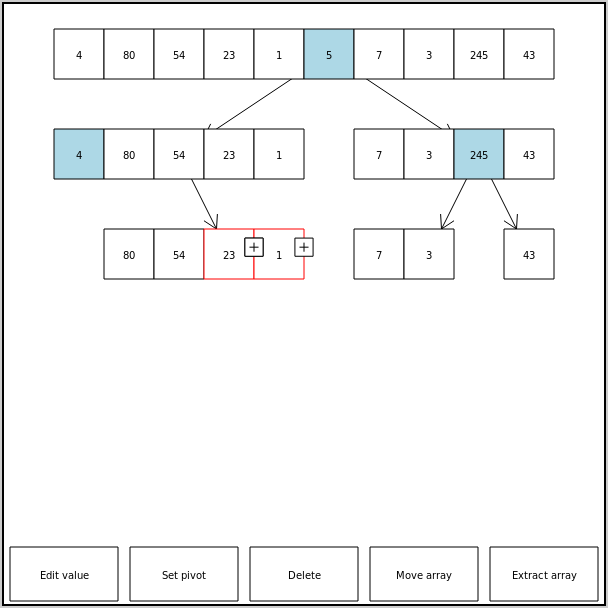
\includegraphics[width=0.75\linewidth]{/graphdrawer/sortui}
    \caption{Sort - user interface}
    \label{fig:graphdrawerSortUserInterface}
\end{figure}
The following properties can be determined by the optional configuration object:
\begin{enumerate}
    \item \code{sortType}, determines which algoritm to use. Can either be \code{"Mergesort"} or \code{"Quicksort"}. The default value is \code{"Quicksort"}.
    \item \code{bsf}, button-size-factor, determines how large the "+" buttons between nodes are. The default value is 3.
    \item \code{pivotColor}, determines which fill color nodes which are marked as pivot will have.
    \item \code{selectedColor}, determines which stroke color nodes which are selected will have.
    \item \code{extractType}, determines node position relative to other nodes when extracting nodes from an array. Possible values are \code{"vSorter"} which means the nodes are positioned based on their value, from low to high, and \code{"xSorter"} which poisitions them based on their x-position in the world.
    \item \code{joinType}, determines node position relative to other nodes when joining the nodes from different arrays to a new array. Possible values are \code{"vSorter"} and \code{"xSorter"}.
    \item \code{steps}, which contains information about the starting array which the student needs to sort. It can also contain information about all of the actions one of the algorithms perform to sort the array.
\end{enumerate}
The \code{mouseDownHandler} function has four parts. It will first check if the world is empty. If it is, the first click will create the first node and array. If it is not empty, then it will check if any of the buttons were clicked. The buttons can only be clicked if they are visible, and they are made visible when the user selects one or more nodes. Only one node can be marked as \code{selected} (marked by + buttons \ref{fig:graphdrawerSortUserInterface}), but several can be in the selection list (marked by a red border \ref{fig:graphdrawerSortUserInterface}). When the user selects a node, the "Edit value", "Set pivot" and "Delete" buttons are shown. If the selection list contains node from only one array, the "Move array" and "Extract array" buttons are also shown. If the \code{sortType} is \code{"Mergesort"} and the selection list contains nodes from at least one array, then the "Join" button is also shown. If no button is clicked, and the user is trying to move an array, the array will be moved to the position of the interaction event. Finally, if nothing else happened, the selected node and the selection list is updated based on which nodes the user interacts with. When the user clicks and holds down their mouse button, the controller will start tracking which nodes are under the cursor. When the button is released, any node which was under the cursor will be in the selection list, and the last node from the list will be the selected node.
\\[11pt]
Arrays doesn't exist in the GraphDrawer world. They are therefore only a part of the Sort controller. The controller has a reference to an array of array objects. The array objects contain a reference to every node in the array, the position of the array, and an list of other arrays which the array has a connection to. When an array is created, its position is set to the position of the first node. This is done so that the array won't move when more nodes are added to it. When a node is added to the array, all of the other nodes in the array will have an invalid position. To fix this, the node is first placed at the correct index, and then every node in the array is positioned according to their index in the reference array. When a node is removed, the same steps are performed. Because arrays doesn't exists in the GraphDrawer, edges between them also doesn't exist. Any link between two arrays, is really an edge between the nodes closest to the center of the arrays. This is achieved by updating the link when a node is added or removed from the array.
\\[11pt]
Even though all the controllers have a property with the name \code{steps}, the format doesn't have to be the same. Graph0 imports and exports the whole state of the graph after every operation. The steps in Sort just contain information about which operation was performed, and on which elements. E.g. \code{{ type: "Split", list: [], left: [], right: [], ...}}. Sort is able to export and parse the following step types: "Initial", "Split", "Merge", "Complete". The initial step is used to describe the starting array. The split and merge steps are used to show what operation was performed, and its result. Because the exported steps also follow this format, it is possible that the student did something which is not considered a valid operation, e.g. split one array to four new arrays. To handle this, the complete step is used. If a student performs an invalid operation, the complete graph (similar to Graph0) is exported instead of an operation. The following is a list of all the required properties for every step type:
\begin{enumerate}
    \item \code{"Initial"}
    \begin{itemize}
        \item \code{list}, contains all the nodes in the array which should be sorted. The list should only contain the node values, because the node objects are created by the import function.
    \end{itemize}
    \item \code{"Split"}
    \begin{itemize}
        \item \code{list}, contains all the nodes in the array which should be split. The list should only contain node values.
        \item \code{left} and \code{right}, contains the nodes which are either placed in the left or the right array. At least one of them is required. One of them can be undefined, because splitting an array on a pivot, might only give one new array if a non-optimal pivot was picked.
        \item \code{pivot}, determines which node is the pivot node. If \code{sortType} is \code{"Mergesort"} this should be \code{undefined}. The student is able to mark more than one node as the pivot, however if that happens, the operation is invalid and the step type will be \code{"Complete"} instead.
    \end{itemize}
    \item \code{"Merge"}
    \begin{itemize}
        \item \code{merged}, contains the result of the merge operation. 
        \item \code{list1}, contains the node values from one of the lists which is being merged.
        \item \code{list2}, contains the node values from the other list which is being merged.
        \item \code{pivot}, if the \code{sortType} is \code{"Quicksort"} this is the node which is used as the pivot for the merge. 
    \end{itemize}
    \item \code{"Complete"}
    \begin{itemize}
        \item \code{arrays}, should be an array containing all of the arrays. This doesn't enforce any restrictions on the arrays, e.g. one array can link to more than two other arrays.
    \end{itemize}
\end{enumerate}

\subsubsection{Dijkstra}
The Dijkstra controller lets user perform Dijkstra's Shortest Path First algorithm on a given graph.
\begin{figure}[H]
    \centering
    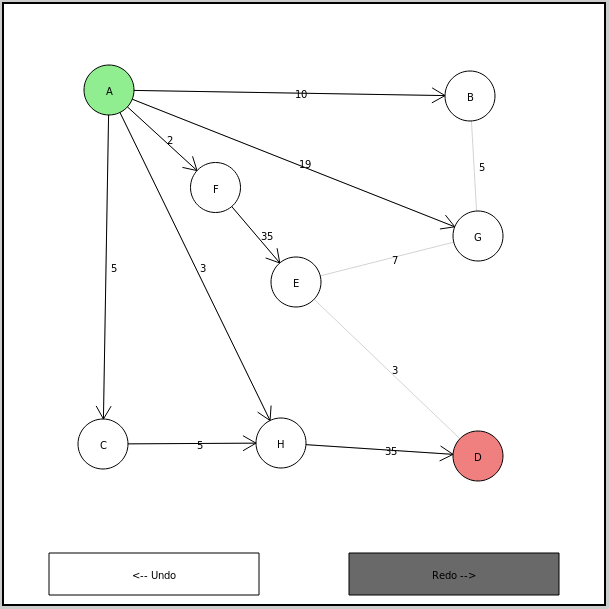
\includegraphics[width=0.7\linewidth]{/graphdrawer/dijkstraui}
    \caption{Dijkstra - user interface}
    \label{fig:graphdrawerDijkstraUserInterface}
\end{figure}
If the Dijkstra controller is not given a configuration object, then it will only display a white screen without allowing any user interaction. This happens becuase this controller is made for finding the shortest path, or for showing how the algorithm finds the shortest path. It can not be used to create a graph. The following properties can be determined by the configuration object:
\begin{enumerate}
    \item \code{steps}, should be an array of the steps the algorithm uses to find the shortest path. This can be undefined, if the intention is for the student to use the algorithm to find the path. If \code{steps} is defined, then the \code{graph} configuration is not needed.
    \item \code{startColor}, the fill color used for the start node.
    \item \code{endColor}, the fill color used for the end node.
    \item \code{edgeColor}, is the color used for lines which show the path between nodes.
    \item \code{graph}, contains information about the graph which the student should use the algorithm on. The following list is all of the possible properties on the \code{graph} object.
    \begin{itemize}
        \item \code{graph}, contains the graph.
        \item \code{from}, should be the starting node.
        \item \code{to}, should be the end node.
        \item \code{nodes}, should be an array of node objects which the graph consists of.
    \end{itemize}
\end{enumerate}
The Dijkstra controller uses the steps array to store operations. There are three step types:
\begin{enumerate}
    \item \code{"Initial"}, is used to store information about the graph. It has the same properties as the \code{graph} configuration object.
    \item \code{"Distance"}, is used to show that the algorithm is checking the cost between to nodes. 
\end{enumerate}

\subsection{Python}
Python is the programming language used in the DAT100 course at UiS. Students are often struggeling to understand the difference between value type and reference type variables. To make it easier for them to learn, a Python interpreter was implemented which evaluates Python code step by step. Together with the GraphDrawer, the interpreter can be used to ask questions about Python code. The student is able to see whether a variable is value or reference type, and they can see when the value or reference changes. Before implementing a custom interpreter, using the offical Python interpreter was considered. Because of the size of CPython, and the limited time available for this project, it was decided that implementing a custom interpreter was the better option.
\\[11pt]
The following features of Python are supported:
\begin{enumerate}
    \item Variables of the following types: Number, String, Boolean, and Object.
    \item Functions can be defined using the \code{def} keyword. They can either belong to the global scope, or to a class. Functions can return something using the \code{return} keyword.
    \item Classes can be defined using the \code{class} keyword. If a function with the \code{__init__} is defined inside the class, it will be called when a new instance of the class is instantiated.
    \item If statements can be used with the \code{if} keyword. Elif and else statements are also supported.
    \item The following mathematical operators are supported: +, -, /, *.
    \item The following comparison operators are supported: and, or, !, ==, !=, <, >, >=, <=.
    \item Expressions can be grouped and seperated using parenthesis.
    \item Lines starting with a # are treated as comments, and will be skipped by the interpreter.
\end{enumerate}
Significant Python features missing from this interpreter:
\begin{enumerate}
    \item The standard library.
    \item Lists and dictionaries.
    \item Inner classes and functions.
    \item Shared class variables.
    \item Class inheritance.
    \item Loops.
\end{enumerate}
Every operator has the same priority, which means that expressions are always evaluated left to right. This makes some expressions not behave like expected. The following statement results in an error: \code{if 1 + 1 == 2:}, because it is evaluated as \code{1 + (1 == 2)}. To prevent this from happening, parenthesis should be used to order the expressions. The correct statement would be: \code{if (1 + 1) == 2:}.

\subsubsection{Interpreter}
There are three main functions in the interpreter. \code{parseLine} which tries to figure out what the meaning of a code line is. \code{parseLine} is also responsible for deciding which line to parse next. A line can either be a variable assignment which is handled  by the \code{parseLine} function, an expression which is handled by the \code{evaluateExpression} function, or a statement which is handled by the \code{handleKeyword} function. A statement is anything which starts with one of the keywords. An expression is something which can be evaluated to a value.
!! Insert fancy image showing the path code goes trough the interpreter !!
\\[11pt]
An important feature of the interpreter is the scope objects. A scope is an object which stores information about the variables, classes, functions and data inside the scope. Functions are scopes because they can contain private variables. Classes are also scopes, because they can contain functions. Before code can be parsed, a global scope is created. Anything which doesn't belong to a specific scope, is placed in the global scope. Scope data is an array where the index is the address of the stored data, and the value is the stored data. Because the interpreter is implemented in JavaScript, there is no need to seperate value and references types in this array because JavaScript and Python behave the same way. Scope variables are a mapping from variable names to data addresses. Scope functions/classes are mappings from function/class names to function/class objects. Because the interpreter should save the state of the program as steps, the \code{parseLine} function returns an object containing information about the state. If the state was anything other than a function or class definition, the current state is saved as a step.
\\[11pt]
A function is an object with a \code{name}, a list of arguments \code{args}, a list of the code lines belonging to the function \code{code}. A function should also be a scope. The name is used to identify the function. The arguments are used to make sure that when the function is called, the right amount of arguments are passed. The code is stored so the function can be evaluated when it is called. After a function has been defined, the \code{handleKeyword} function returns a state of type \code{"SkipLines"} which tells the caller which lines have already been handled. The interpreter uses the \code{callFunc} function to call Python functions. When a function is called, three things happen in the following order:
\begin{enumerate}
    \item The function arguments are added as local variables. Local variables mean they belong to the function scope. The arguments need to be in the same order as they were defined, because named arguments are not implemented.
    \item Every line found in the functions \code{code} list is parsed using \code{parseLine}. If a \code{return} statement is found before reaching the end, the function will stop parsing, before reaching the end.
    \item The scope of the function is restored to an empty state and data is returned if a return statement was found.
\end{enumerate}
\\[11pt]
A class is an object with a \code{name} and a list of the code lines belonging to the class \code{code}. A class should also be a scope. When a class is defined, the code is also parsed using the \code{parseLine} function. This is done so that any functions within the class is defined in the scope of the class. When the interpreter is instantiating an instance of the class, the \code{instantiateClass} function is called. \code{instantiateClass} will first create a new object which contains all the functions from the class. If the class has a constructor it is called. Finally, the object is returned to the called of \code{instantiateClass}.
!! Write about expression evaluation !!
!! Write about operators !!

\subsubsection{Questions}
!! TODO: Write this :=) !!
